\chapter{Simetría y leyes de conservación}

\lectureoverview{La acción estacionaria y las ecuaciones de Euler--Lagrange constituyen una mitad del núcleo de la mecánica clásica; la formulación hamiltoniana constituye la otra. Aquí desarrollaremos la primera lo suficiente para revelar un patrón profundo: toda simetría continua de un lagrangiano produce una cantidad conservada. Descubriremos el patrón mediante traslaciones y rotaciones, lo demostraremos para una transformación infinitesimal general y examinaremos después con cuidado dónde se aplica el argumento y dónde no.}

\section{Las matemáticas mínimas que explican la física}

Las expresiones que ya están en la pizarra quizá recuerden un poco a la ecuación de Schrödinger, pero ese no es el tema de hoy. El tema es la simetría y la conservación. No hay una manera honesta de explicar su relación sin ecuaciones. Las ecuaciones son elementales; lo importante es organizarlas para que la estructura se haga visible. Scientific American quizá dé nombre al resultado, pero aquí buscamos las matemáticas mínimas necesarias para deducirlo como lo harían los físicos.

Introduzcamos un parámetro pequeño \(\epsilon\). Conservamos los términos proporcionales a \(\epsilon\) y descartamos \(O(\epsilon^2)\). Esta es una abreviatura de un argumento de límite, no la afirmación de que el cuadrado de un número real no nulo sea literalmente cero. Para una función ordinaria \(f(x,y)\),
\begin{equation}
  \delta f
  =\frac{\partial f}{\partial x}\,\delta x
   +\frac{\partial f}{\partial y}\,\delta y
   +O(\epsilon^2),
  \label{eq:first-variation-f}
\end{equation}
donde tanto \(\delta x\) como \(\delta y\) son proporcionales a \(\epsilon\). El símbolo \(\delta f\) representa el cambio de \(f\), no el producto de un número llamado \(\delta\) por \(f\). En un punto estacionario se cumple
\begin{equation}
  \delta f=0
  \qquad\hbox{to first order.}
  \label{eq:stationary-f}
\end{equation}

Para una trayectoria mecánica \(q_i(t)\), la cantidad análoga es la acción
\begin{equation}
  S[q]=\int_{t_1}^{t_2}L(q,\dot q,t)\,dt.
  \label{eq:action-l4}
\end{equation}
Al variar la trayectoria manteniendo fijos sus extremos, se obtiene
\begin{equation}
  \delta S
  =\int_{t_1}^{t_2}dt\,
   \sum_i\left(
     \frac{\partial L}{\partial q_i}\,\delta q_i
     +\frac{\partial L}{\partial\dot q_i}\,\delta\dot q_i
   \right).
  \label{eq:action-variation-l4}
\end{equation}
Los dos términos aparecen porque al cambiar la trayectoria cambian tanto su posición como su velocidad. La integración por partes, junto con
\(\delta q_i(t_1)=\delta q_i(t_2)=0\), transforma \(\delta S=0\) en
\begin{equation}
  \frac{d}{dt}\left(\frac{\partial L}{\partial\dot q_i}\right)
  -\frac{\partial L}{\partial q_i}=0.
  \label{eq:el-l4}
\end{equation}

\begin{figure}[htbp]
  \centering
  \includegraphics[width=0.76\textwidth]{lecture_04_figure_05.png}
  \caption{La ecuación de Euler--Lagrange, recordada como punto de partida para estudiar la simetría y la conservación.}
  \lectureframe{00:09:00}
\end{figure}

La expresión correcta es \emph{acción estacionaria}, no necesariamente acción mínima. Retomaremos esta distinción hacia el final.

\section{Coordenadas generalizadas y momento conjugado}

Las posiciones cartesianas son un lenguaje demasiado limitado para la mecánica general. Las coordenadas pueden ser posiciones de partículas, ángulos, variables colectivas o amplitudes de campo; por eso las llamamos \(q_i\). Un lagrangiano es una especificación compacta de la dinámica. Incluso el Modelo Estándar, escrito sin una notación muy condensada, ocupa aproximadamente una página; escribir una ecuación de movimiento independiente para cada componente de campo ocuparía muchísimo más. La única función \(L\) los engloba a todos.

El momento conjugado a \(q_i\) es
\begin{equation}
  p_i=\frac{\partial L}{\partial\dot q_i}.
  \label{eq:canonical-momentum-l4}
\end{equation}
Por eso tradicionalmente se llama a las coordenadas generalizadas \(q\) y a los momentos correspondientes \(p\): así obtenemos nuestras \(p\) y nuestros \(q\). Con esta notación, la ec.~\eqref{eq:el-l4} queda
\begin{equation}
  \dot p_i=\frac{\partial L}{\partial q_i}.
  \label{eq:momentum-el-l4}
\end{equation}

Para la conocida partícula unidimensional,
\begin{equation}
  L=\frac{m\dot x^2}{2}-V(x),
  \qquad
  \frac{\partial L}{\partial\dot x}=m\dot x,
  \label{eq:particle-momentum-l4}
\end{equation}
por lo que el momento conjugado es el momento lineal ordinario.

\begin{figure}[htbp]
  \centering
  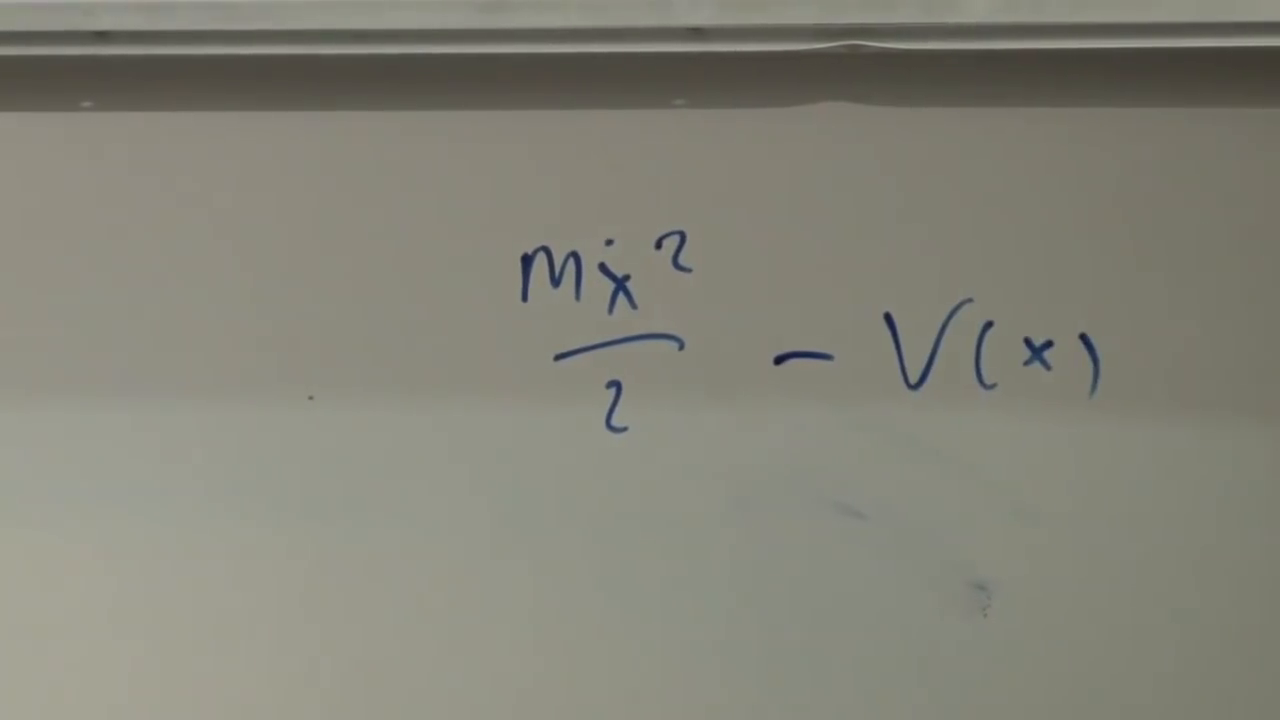
\includegraphics[width=0.72\textwidth]{lecture_04_figure_02.png}
  \caption{El lagrangiano, energía cinética menos energía potencial, que permite identificar el momento conjugado con \(m\dot x\).}
  \lectureframe{00:14:48}
\end{figure}

Si \(q_i\) no aparece en \(L\), entonces \(\dot p_i=0\). Esta es la conocida vía de la coordenada cíclica para obtener una ley de conservación. La conexión real es más general, y conviene descubrirla con ejemplos antes de demostrarla.

\section{Leyes de conservación descubiertas antes de explicarlas}

\subsection{Dos coordenadas y un potencial que depende de su diferencia}

Tomemos ambas masas iguales a uno y consideremos
\begin{equation}
  L=\frac{\dot q_1^{\,2}+\dot q_2^{\,2}}{2}-V(q_1-q_2).
  \label{eq:separation-lagrangian}
\end{equation}
Podemos imaginar dos partículas sobre una recta. Su interacción depende únicamente de la separación entre ellas.

\begin{figure}[htbp]
  \centering
  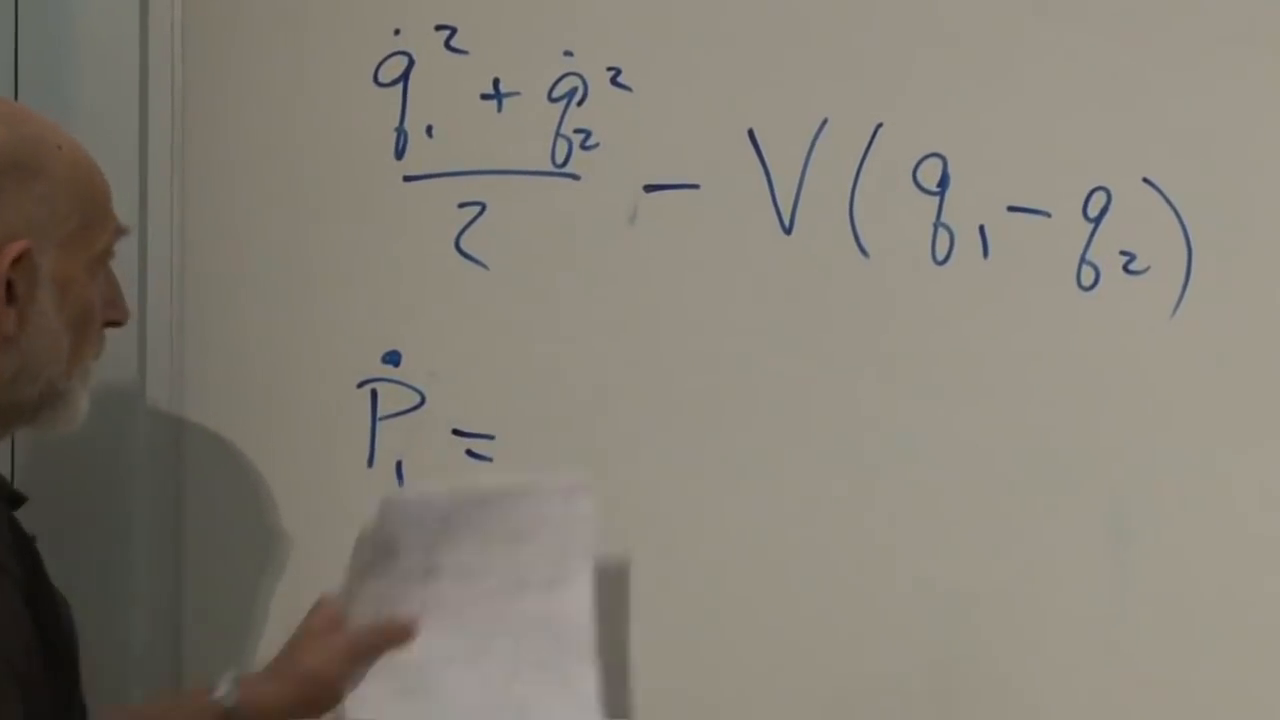
\includegraphics[width=0.78\textwidth]{lecture_04_figure_03.png}
  \caption{El lagrangiano de dos coordenadas y el comienzo de la primera ecuación para el momento.}
  \lectureframe{00:18:56}
\end{figure}

Escribiendo \(V'\) para la derivada respecto del argumento de \(V\),
\begin{align}
  \dot p_1&=-V'(q_1-q_2),
  \notag\\
  \dot p_2&=+V'(q_1-q_2).
  \label{eq:separation-momentum-equations}
\end{align}
El signo de la segunda ecuación se invierte porque al aumentar \(q_2\) disminuye \(q_1-q_2\).

\begin{classroomqa}
  \audiencequestion{¿Debe aparecer \(V'\) en la primera ecuación para el momento, y de dónde viene su signo menos?
  \lecturetimestamp{00:20:52--00:21:35}}
  \lecturerresponse{La ecuación de Euler--Lagrange establece que
  \(\dot p_1=\partial L/\partial q_1\), no que el lagrangiano sea cero.
  Como \(L=T-V\), al derivar respecto de \(q_1\) se obtiene
  \(-V'\). Al derivar respecto de \(q_2\) aparece otro signo menos debido a \(q_1-q_2\), así que la segunda ecuación contiene \(+V'\).}
\end{classroomqa}

\begin{figure}[htbp]
  \centering
  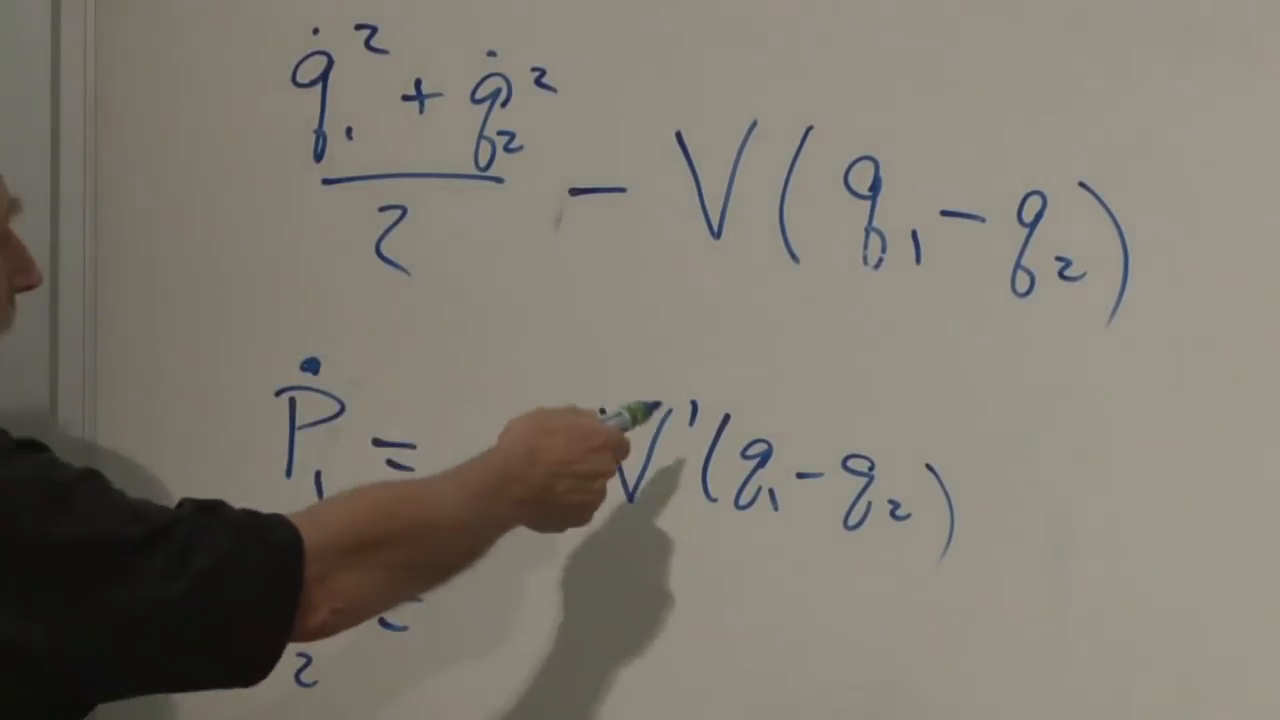
\includegraphics[width=0.78\textwidth]{lecture_04_figure_04.png}
  \caption{La derivada cuyo signo hay que cuidar en la ecuación de \(p_1\); en la ecuación de \(p_2\) aparece el signo opuesto.}
  \lectureframe{00:20:41}
\end{figure}

Al sumar las ecs.~\eqref{eq:separation-momentum-equations} se obtiene
\begin{equation}
  \frac{d}{dt}(p_1+p_2)=0.
  \label{eq:total-p-conserved}
\end{equation}
Hemos encontrado una cantidad conservada, pero aún no hemos explicado por qué existe.

\subsection{Una combinación lineal menos evidente}

Consideremos ahora
\begin{equation}
  L=\frac{\dot q_1^{\,2}+\dot q_2^{\,2}}{2}
    -V(Aq_1+Bq_2),
  \label{eq:ab-lagrangian}
\end{equation}
donde \(A\) y \(B\) son constantes. Entonces
\begin{align}
  \dot p_1&=-A\,V'(Aq_1+Bq_2),
  \notag\\
  \dot p_2&=-B\,V'(Aq_1+Bq_2).
  \label{eq:ab-momentum-equations}
\end{align}
Multiplicando la primera ecuación por \(B\), la segunda por \(A\) y restándolas, se elimina la fuerza:
\begin{equation}
  \frac{d}{dt}(Bp_1-Ap_2)=0.
  \label{eq:ab-conserved}
\end{equation}

\begin{figure}[htbp]
  \centering
  \includegraphics[width=0.78\textwidth]{lecture_04_figure_06.png}
  \caption{Las ecuaciones ponderadas para los momentos, cuyos términos de fuerza se cancelan en \(Bp_1-Ap_2\).}
  \lectureframe{00:24:20}
\end{figure}

\begin{classroomqa}
  \audiencequestion{¿Qué origen físico podrían tener constantes como \(A\) y \(B\)?
  \lecturetimestamp{00:25:09--00:30:15}}
  \lecturerresponse{Consideremos dos partículas de masas \(m\) y \(M\):
  \[
    L=\frac{m\dot X^2}{2}+\frac{M\dot Y^2}{2}-V(X-Y).
  \]
  Hagamos el cambio de escala \(Q_1=\sqrt m\,X\) y \(Q_2=\sqrt M\,Y\). El término cinético se convierte en \((\dot Q_1^2+\dot Q_2^2)/2\), mientras que el potencial depende de \(Q_1/\sqrt m-Q_2/\sqrt M\). Así, las masas desiguales se convierten de forma natural en coeficientes de una combinación lineal. Sustituir \(Q_2\) por \(-Q_2\) cambia el signo menos mostrado por un signo más, sin alterar el término cinético al cuadrado.}
\end{classroomqa}

\begin{figure}[htbp]
  \centering
  \includegraphics[width=0.82\textwidth]{lecture_04_figure_07.png}
  \caption{Las coordenadas ponderadas por la masa simplifican la energía cinética y trasladan los factores de masa al potencial.}
  \lectureframe{00:28:40}
\end{figure}

\begin{classroomqa}
  \audiencequestion{¿Esto demuestra que puede existir una cantidad conservada sin una coordenada cíclica?
  \lecturetimestamp{00:31:13--00:31:58}}
  \lecturerresponse{En las variables tal como están escritas no hay ninguna coordenada cíclica \emph{evidente}. Un cambio de variables puede revelarla, pero buscarla no es aquí el enfoque más útil. El argumento de simetría identificará directamente la combinación conservada.}
\end{classroomqa}

\section{Qué entendemos por simetría}

\subsection{Traslaciones}

Empecemos con una partícula libre de masa unitaria,
\begin{equation}
  L=\frac{\dot q^2}{2}.
  \label{eq:free-unit-l4}
\end{equation}
Traslademos todos los puntos de su historia en la misma cantidad constante:
\begin{equation}
  q'(t)=q(t)+\epsilon.
  \label{eq:free-translation}
\end{equation}
Como \(\epsilon\) es independiente del tiempo, \(\dot q'=\dot q\) y, por tanto,
\(\delta L=0\). Esta invariancia es la simetría de traslación.

Hay dos descripciones equivalentes. En la descripción pasiva, desplazamos el origen de coordenadas y dejamos el objeto fijo. En la activa, mantenemos fijos los ejes y movemos el objeto. El lenguaje activo resulta menos confuso: movemos la configuración física y preguntamos si \(L\) lo detecta.

Para la ec.~\eqref{eq:separation-lagrangian}, traslademos ambas coordenadas:
\begin{equation}
  \delta q_1=\epsilon,
  \qquad
  \delta q_2=\epsilon.
  \label{eq:common-translation}
\end{equation}
Las velocidades no cambian, y \(q_1-q_2\) tampoco.

\begin{figure}[htbp]
  \centering
  \includegraphics[width=0.78\textwidth]{lecture_04_figure_08.png}
  \caption{Una traslación común deja inalterada la separación entre dos coordenadas.}
  \lectureframe{00:35:30}
\end{figure}

Para la ec.~\eqref{eq:ab-lagrangian}, usemos la transformación menos evidente
\begin{equation}
  \delta q_1=B\epsilon,
  \qquad
  \delta q_2=-A\epsilon.
  \label{eq:ab-transformation}
\end{equation}
De nuevo, las velocidades no cambian, mientras que
\begin{equation}
  \delta(Aq_1+Bq_2)=AB\epsilon-BA\epsilon=0.
  \label{eq:ab-invariant-argument}
\end{equation}
Así pues, esta transformación es una simetría.

\begin{figure}[htbp]
  \centering
  \includegraphics[width=0.80\textwidth]{lecture_04_figure_09.png}
  \caption{La traslación asimétrica que conserva \(Aq_1+Bq_2\).}
  \lectureframe{00:40:20}
\end{figure}

\begin{classroomqa}
  \audiencequestion{¿Los coeficientes codifican las masas, de modo que la cantidad conservada se convierte en el momento lineal ordinario del centro de masas?
  \lecturetimestamp{00:42:25--00:42:45}}
  \lecturerresponse{Sí. En las variables ponderadas por la masa, la simetría y la combinación conservada parecen asimétricas. Al volver a \(X\) y \(Y\) se recuperan la traslación simultánea ordinaria y el momento lineal total.}
\end{classroomqa}

\subsection{Rotaciones}

Consideremos una partícula en el plano,
\begin{equation}
  L=\frac{m}{2}(\dot x^2+\dot y^2)-V(x^2+y^2).
  \label{eq:central-lagrangian-l4}
\end{equation}
Se trata de un potencial central. Comparamos dos sistemas de coordenadas fijos, girados uno respecto del otro; los ejes no están girando con el tiempo. Con una orientación coherente,
\begin{align}
  x'&=x\cos\theta+y\sin\theta,
  \notag\\
  y'&=-x\sin\theta+y\cos\theta.
  \label{eq:finite-rotation-l4}
\end{align}

\begin{figure}[htbp]
  \centering
  \includegraphics[width=0.82\textwidth]{lecture_04_figure_10.png}
  \caption{Un lagrangiano con potencial central y dos marcos cartesianos fijos relacionados mediante una rotación.}
  \lectureframe{00:45:40}
\end{figure}

Tomemos \(\theta=\epsilon\) y conservemos solo el primer orden:
\begin{equation}
  \cos\epsilon=1+O(\epsilon^2),
  \qquad
  \sin\epsilon=\epsilon+O(\epsilon^3).
  \label{eq:small-angle-l4}
\end{equation}
La rotación infinitesimal es
\begin{align}
  \delta x&=y\epsilon,
  &\delta y&=-x\epsilon,
  \notag\\
  \delta\dot x&=\dot y\epsilon,
  &\delta\dot y&=-\dot x\epsilon.
  \label{eq:infinitesimal-rotation-l4}
\end{align}

\begin{figure}[htbp]
  \centering
  \includegraphics[width=0.82\textwidth]{lecture_04_figure_11.png}
  \caption{La rotación infinitesimal de las coordenadas y las velocidades.}
  \lectureframe{00:49:50}
\end{figure}

A diferencia de lo que ocurre con una traslación, la magnitud del cambio de \(x\) depende de \(y\), y la del cambio de \(y\) depende de \(x\). Sin embargo,
\begin{align}
  \delta(x^2+y^2)
  &=2x\,\delta x+2y\,\delta y=0,
  \notag\\
  \delta(\dot x^2+\dot y^2)
  &=2\dot x\,\delta\dot x+2\dot y\,\delta\dot y=0.
  \label{eq:rotation-invariants-l4}
\end{align}
Tanto el término potencial como el cinético son invariantes.

\begin{figure}[htbp]
  \centering
  \includegraphics[width=0.76\textwidth]{lecture_04_figure_12.png}
  \caption{La cancelación de primer orden que demuestra la invariancia del radio al cuadrado bajo rotaciones.}
  \lectureframe{00:53:20}
\end{figure}

\section{El teorema general de conservación}

Los ejemplos de traslación y rotación comparten una misma forma. Sea una transformación continua infinitesimal
\begin{equation}
  \delta q_i=\epsilon f_i(q),
  \qquad
  \delta\dot q_i=\frac{d}{dt}\delta q_i,
  \label{eq:general-infinitesimal-symmetry}
\end{equation}
donde \(\epsilon\) es independiente del tiempo y \(f_i\) puede depender de todas las coordenadas.

\begin{figure}[htbp]
  \centering
  \includegraphics[width=0.78\textwidth]{lecture_04_figure_13.png}
  \caption{Un campo general de desplazamientos infinitesimales \(\delta q_i=\epsilon f_i(q)\).}
  \lectureframe{00:56:00}
\end{figure}

La variación de primer orden del lagrangiano es
\begin{equation}
  \delta L
  =\sum_i\left(
    \frac{\partial L}{\partial q_i}\delta q_i
    +\frac{\partial L}{\partial\dot q_i}\delta\dot q_i
  \right).
  \label{eq:delta-l-general}
\end{equation}

\begin{figure}[htbp]
  \centering
  \includegraphics[width=0.84\textwidth]{lecture_04_figure_14.png}
  \caption{Las dos contribuciones a \(\delta L\): la variación de las coordenadas y la variación de las velocidades.}
  \lectureframe{01:02:30}
\end{figure}

Restringimos ahora la atención a una trayectoria física, de modo que se cumplen las ecuaciones de Euler--Lagrange. Usando
\begin{equation}
  \frac{\partial L}{\partial\dot q_i}=p_i,
  \qquad
  \frac{\partial L}{\partial q_i}=\dot p_i,
  \label{eq:el-substitution-l4}
\end{equation}
obtenemos
\begin{align}
  \delta L
  &=\sum_i\left(\dot p_i\,\delta q_i
                +p_i\,\delta\dot q_i\right)
  \notag\\
  &=\frac{d}{dt}\sum_i p_i\delta q_i
  =\epsilon\frac{d}{dt}\sum_i p_i f_i(q).
  \label{eq:noether-derivation-l4}
\end{align}
El paso central consiste únicamente en aplicar la regla del producto.

Si la transformación es una simetría, \(\delta L=0\). Como \(\epsilon\) es un factor constante arbitrario,
\begin{equation}
  \boxed{
  \frac{d\mathcal Q}{dt}=0,
  \qquad
  \mathcal Q=\sum_i p_i f_i(q)}
  .
  \label{eq:noether-charge-l4}
\end{equation}
Este es el núcleo de la versión de la mecánica clásica del teorema de Noether para simetrías puntuales exactas e independientes del tiempo.

\begin{figure}[htbp]
  \centering
  \includegraphics[width=0.84\textwidth]{lecture_04_figure_15.png}
  \caption{El paso de la regla del producto que convierte la invariancia de \(L\) en una cantidad conservada.}
  \lectureframe{01:05:00}
\end{figure}

\begin{classroomqa}
  \audiencequestion{En \(f_i(q)\), ¿\(q\) lleva otro índice?
  \lecturetimestamp{01:06:57--01:07:31}}
  \lecturerresponse{El símbolo \(q\) sin índice denota el conjunto completo \((q_1,q_2,\ldots)\). Cada componente \(f_i\) puede depender de todas esas coordenadas. Por ejemplo, para una rotación, \(f_x=y\) y \(f_y=-x\).}
\end{classroomqa}

Los ejemplos ya no parecen casos accidentales. Para una traslación común, \(f_1=f_2=1\), así que
\begin{equation}
  \mathcal Q=p_1+p_2.
  \label{eq:noether-common-p}
\end{equation}
Para la traslación asimétrica, \(f_1=B\), \(f_2=-A\), así que
\begin{equation}
  \mathcal Q=Bp_1-Ap_2.
  \label{eq:noether-ab-p}
\end{equation}
Para una rotación, \(f_x=y\) y \(f_y=-x\):
\begin{equation}
  \mathcal Q=p_xy-p_yx.
  \label{eq:rotation-charge-sign}
\end{equation}
Salvo por el signo que depende de la orientación, esto es el momento angular,
\begin{equation}
  J=xp_y-yp_x.
  \label{eq:angular-momentum-l4}
\end{equation}

\begin{figure}[htbp]
  \centering
  \includegraphics[width=0.82\textwidth]{lecture_04_figure_16.png}
  \caption{La carga de Noether para la rotación, igual al momento angular en el plano salvo por el signo asociado a la orientación.}
  \lectureframe{01:11:00}
\end{figure}

Para muchas partículas que interactúan, hagamos girar todas a la vez. La invariancia conserva entonces la suma de sus momentos angulares, no el momento angular de cada partícula por separado.

\section{Preguntas sobre las hipótesis del teorema}

\begin{classroomqa}
  \audiencequestion{¿Un conjunto de ejes que gira introduciría dependencia explícita del tiempo en \(\delta L\)?
  \lecturetimestamp{01:12:57--01:13:57}}
  \lecturerresponse{Sí. La demostración anterior supone un parámetro de simetría independiente del tiempo: una traslación fija o una rotación fija. Una transformación cuyo parámetro depende del tiempo produce términos adicionales y requiere un tratamiento más general.}
\end{classroomqa}

\begin{classroomqa}
  \audiencequestion{¿La letra mayúscula \(Q\) de la fórmula de la pizarra representa la transformación misma?
  \lecturetimestamp{01:14:02--01:15:58}}
  \lecturerresponse{No. Por desgracia, esa notación coincide con la de las coordenadas \(q_i\). La transformación es \(\delta q_i=\epsilon f_i(q)\); la cantidad conservada que resulta es \(\mathcal Q=\sum_i p_i f_i\). El coeficiente \(f_i\) indica cómo se desplaza bajo la simetría la coordenada \(i\).}
\end{classroomqa}

La conservación de la energía también se debe a una simetría, pero a otra distinta: la traslación temporal, o la independencia respecto de dónde se sitúe el origen del tiempo. Dejamos ese caso y la formulación hamiltoniana para más adelante.

\begin{classroomqa}
  \audiencequestion{¿Podría incorporarse el movimiento real mediante un sistema de coordenadas cambiante, de modo que la mecánica no fuera más que transformaciones de coordenadas?
  \lecturetimestamp{01:17:43--01:20:01}}
  \lecturerresponse{Se pueden elegir coordenadas que acompañen un movimiento particular, pero entonces la transformación depende del estado inicial y de la trayectoria. La transformación de simetría que usamos aquí se fija independientemente de la solución que siga el sistema. El movimiento en sí se representa de forma más natural en el espacio conjunto de coordenadas y momentos.}
\end{classroomqa}

\section{El oscilador armónico en el espacio de fases}

Tomando la masa y la constante del resorte iguales a uno,
\begin{equation}
  L=\frac{\dot q^2}{2}-\frac{q^2}{2}.
  \label{eq:oscillator-l4}
\end{equation}
El momento conjugado y la ecuación de movimiento dan
\begin{equation}
  p=\dot q,
  \qquad
  \dot p=-q,
  \label{eq:oscillator-first-order-l4}
\end{equation}
o, equivalentemente,
\begin{equation}
  \dot q=p,
  \qquad
  \dot p=-q.
  \label{eq:oscillator-phase-flow}
\end{equation}
Estas ecuaciones describen un movimiento circular uniforme en el plano \(q\)-\(p\). El oscilador que va y viene en el espacio real es la proyección de ese círculo sobre el eje \(q\): la rapidez es máxima en \(q=0\) y se anula en los puntos de retorno.

\begin{figure}[htbp]
  \centering
  \includegraphics[width=0.82\textwidth]{lecture_04_figure_17.png}
  \caption{Las ecuaciones del oscilador armónico y su órbita circular en el espacio \(q\)-\(p\).}
  \lectureframe{01:25:30}
\end{figure}

\begin{classroomqa}
  \audiencequestion{¿El círculo del espacio de fases se recorre en sentido horario?
  \lecturetimestamp{01:25:47--01:27:15}}
  \lecturerresponse{Sí, si \(p\) es el eje horizontal y \(q\) el vertical. Cuando \(q\) es máximamente positivo, \(\dot p=-q<0\), así que el movimiento apunta hacia abajo. Si se invierte la disposición de los ejes, se invierte el sentido visual; por eso es fácil recordar mal la convención.}
\end{classroomqa}

El par de ecuaciones de la ec.~\eqref{eq:oscillator-phase-flow} ya se parece a las ecuaciones de Hamilton, pero se ha obtenido íntegramente dentro de la mecánica lagrangiana.

\section{Simetrías continuas y discretas}

\begin{classroomqa}
  \audiencequestion{¿Es necesario expresar una simetría mediante una transformación infinitesimal cartesiana?
  \lecturetimestamp{01:27:48--01:30:31}}
  \lecturerresponse{Las coordenadas cartesianas son solo una conveniencia; para esta demostración, el requisito esencial es la continuidad. Algunas simetrías no tienen versión infinitesimal. Si el potencial es par, la reflexión transforma \(q\mapsto -q\) y \(\dot q\mapsto-\dot q\), y deja \(L\) inalterado; pero una reflexión no puede componerse a partir de reflexiones arbitrariamente pequeñas. Por lo tanto, esta derivación clásica no produce ninguna cantidad conservada asociada.}
\end{classroomqa}

\begin{figure}[htbp]
  \centering
  \includegraphics[width=0.82\textwidth]{lecture_04_figure_18.png}
  \caption{Un potencial par es invariante bajo la reflexión discreta \(q\mapsto -q\).}
  \lectureframe{01:29:30}
\end{figure}

\begin{classroomqa}
  \audiencequestion{Si la cantidad conservada \(\mathcal Q\) no es cero, ¿demuestra eso que la transformación no era una simetría?
  \lecturetimestamp{01:30:40--01:31:30}}
  \lecturerresponse{No. Una cantidad conservada puede tener cualquier valor constante. El criterio pertinente es \(\dot{\mathcal Q}\). Si la cantidad deducida de una transformación propuesta no se conserva, entonces esa transformación no era una simetría bajo las hipótesis de la demostración.}
\end{classroomqa}

\begin{classroomqa}
  \audiencequestion{La reflexión sigue dejando inalterado el lagrangiano; ¿por qué no da lugar a una ley de conservación?
  \lecturetimestamp{01:31:34--01:32:27}}
  \lecturerresponse{La invariancia por sí sola es evidente, pero la derivación pasó por un desplazamiento de primer orden y la regla del producto. La reflexión lleva de un lado del espacio de configuraciones al otro en un único paso discreto. Al no haber un generador infinitesimal \(f_i\), la fórmula \(\mathcal Q=\sum_i p_i f_i\) no tiene nada que utilizar.}
\end{classroomqa}

\begin{classroomqa}
  \audiencequestion{¿Cómo se llama la propiedad de poder construirse mediante transformaciones arbitrariamente pequeñas?
  \lecturetimestamp{01:32:36--01:33:23}}
  \lecturerresponse{Se llama \emph{simetría continua}. La traslación y la rotación son continuas; la reflexión es una \emph{simetría discreta}.}
\end{classroomqa}

\begin{classroomqa}
  \audiencequestion{Si muchos pasos infinitesimales forman una transformación finita, ¿pueden acumularse los errores \(O(\epsilon^2)\) descartados?
  \lecturetimestamp{01:33:23--01:36:10}}
  \lecturerresponse{La invariancia infinitesimal debe cumplirse en cada punto al que se llega durante la transformación, no solo en el punto de partida. Dividamos un intervalo finito del parámetro en \(N\) pasos de tamaño \(\epsilon\): el desplazamiento de primer orden acumulado es \(N\epsilon\), mientras que un residuo local \(O(\epsilon^2)\) se acumula como \(N\epsilon^2=(N\epsilon)\epsilon\to0\). Esta estructura de lo local a lo finito es la que formalizan los grupos continuos de transformaciones.}
\end{classroomqa}

\begin{classroomqa}
  \audiencequestion{¿Se realizan físicamente simetrías discretas en sistemas clásicos?
  \lecturetimestamp{01:36:32--01:37:25}}
  \lecturerresponse{Por supuesto. El propio oscilador armónico tiene el potencial par \(V(q)\propto q^2\), por lo que es invariante bajo \(q\mapsto -q\). Hay muchos ejemplos de este tipo; el único punto es que esta invariancia discreta no aporta una nueva carga clásica de Noether.}
\end{classroomqa}

\begin{classroomqa}
  \audiencequestion{Pero si las transformaciones continuas y las discretas dejan inalterado \(L\), ¿no se trata de la misma condición?
  \lecturetimestamp{01:37:37--01:39:18}}
  \lecturerresponse{Es la misma afirmación finita de invariancia, pero no el mismo dato matemático para esta demostración. La demostración necesita una variación de primer orden. En una reflexión, «primer orden» no tiene sentido; por eso ni siquiera se puede iniciar la cadena de ecuaciones que conduce a una carga.}
\end{classroomqa}

\begin{classroomqa}
  \audiencequestion{¿Cuál es la relación histórica con el teorema de Noether?
  \lecturetimestamp{01:39:26--01:40:42}}
  \lecturerresponse{Esta es una parte restringida del teorema mucho más general de Emmy Noether. Ya antes se conocían vínculos particulares entre simetrías y cantidades conservadas, pero a principios del siglo XX Noether los reunió en un marco unificado y notablemente general. La importancia de sus aportaciones matemáticas no se vio correspondida con un trato académico justo.}
\end{classroomqa}

\begin{classroomqa}
  \audiencequestion{¿Sigue siendo la mecánica clásica un campo activo de investigación?
  \lecturetimestamp{01:40:47--01:42:37}}
  \lecturerresponse{Sí. El teorema elemental que usamos aquí es antiguo, pero la dinámica no lineal, los sistemas integrables, el caos, los fluidos y la mecánica geométrica siguen siendo campos de gran riqueza. El principio de simetría también tiene un alcance que va mucho más allá de la mecánica clásica de partículas.}
\end{classroomqa}

\section{Por qué importa el principio de acción}

\begin{classroomqa}
  \audiencequestion{¿Hay una razón intuitiva por la que la simetría debería implicar conservación?
  \lecturetimestamp{01:42:49--01:47:57}}
  \lecturerresponse{La simetría por sí sola no basta para explicarlo. Consideremos el rozamiento viscoso,
  \[
    m\ddot x=-c\dot x.
  \]
  La ecuación es invariante bajo \(x\mapsto x+\epsilon\); sin embargo, con \(p=m\dot x\),
  \[
    \dot p=-\frac{c}{m}p,
    \qquad
    p(t)=p(0)e^{-ct/m},
  \]
  por lo que el momento lineal decae. Esta es una ecuación efectiva para un subsistema, no una ley fundamental de acción estacionaria para \(x\) por sí solo. Si incluimos las moléculas del fluido y el resto del sistema cerrado, el momento lineal total se conserva. La simetría y la conservación están vinculadas mediante el principio lagrangiano de acción, no por la forma de una ecuación diferencial considerada por sí sola.}
\end{classroomqa}

\begin{figure}[htbp]
  \centering
  \includegraphics[width=0.65\textwidth]{lecture_04_figure_19.png}
  \caption{El rozamiento viscoso invariante bajo traslaciones, cuyo momento lineal reducido de la partícula, aun así, decae.}
  \lectureframe{01:44:30}
\end{figure}

\begin{classroomqa}
  \audiencequestion{¿Podemos cuantificar cuándo la trayectoria física no es un mínimo de la acción?
  \lecturetimestamp{01:48:08--01:51:38}}
  \lecturerresponse{Un mínimo verdadero es excepcional; en general, la acción tiene un punto de silla en el espacio de trayectorias. Para el oscilador unitario,
  \[
    S[q]=\frac12\int(\dot q^2-q^2)\,dt.
  \]
  Una deformación estrecha y rápidamente cambiante aumenta la contribución positiva \(\dot q^2\). Una deformación amplia que permanece ligeramente desplazada durante mucho tiempo puede hacer que predomine la contribución negativa \(-q^2\) y reducir la acción. Por tanto, la misma trayectoria estacionaria tiene direcciones en las que la acción aumenta y otras en las que disminuye. La mecánica cuántica, mediante el enfoque de las integrales de trayectoria, ofrece una explicación más profunda de la estacionariedad, pero dejaremos ese argumento para más adelante.}
\end{classroomqa}

\begin{figure}[htbp]
  \centering
  \includegraphics[width=0.80\textwidth]{lecture_04_figure_20.png}
  \caption{Una trayectoria cercana y amplia del oscilador ilustra por qué la acción estacionaria suele corresponder a un punto de silla y no a un mínimo.}
  \lectureframe{01:50:20}
\end{figure}

\begin{classroomqa}
  \audiencequestion{¿Existe una correspondencia biunívoca entre las simetrías continuas y las leyes de conservación?
  \lecturetimestamp{01:51:44--01:52:43}}
  \lecturerresponse{Dentro del marco variacional y una vez identificados los casos equivalentes o triviales, esa es, en esencia, la imagen correcta. Toda simetría continua tiene una carga, y, por lo general, las cantidades conservadas pueden relacionarse con simetrías. Las formulaciones precisas incluyen salvedades técnicas, así que no conviene emplear esta afirmación general sin cuidado.}
\end{classroomqa}

\begin{classroomqa}
  \audiencequestion{¿Debe poseer todo lagrangiano una simetría no trivial?
  \lecturetimestamp{01:52:43--01:53:23}}
  \lecturerresponse{No. Los ejemplos se eligieron precisamente porque tenían simetrías. Un lagrangiano genérico no tiene por qué ser invariante bajo una transformación espacial propuesta.}
\end{classroomqa}

\begin{classroomqa}
  \audiencequestion{¿Debería entenderse finalmente una simetría como un movimiento activo o como un cambio pasivo de coordenadas?
  \lecturetimestamp{01:53:25--01:55:08}}
  \lecturerresponse{Ambas descripciones pueden hacerse equivalentes, pero aquí la activa es más clara. Movemos todo el sistema físico y preguntamos si cambia el lagrangiano. En el lenguaje pasivo, en cambio, hay que decir que la \emph{forma} del lagrangiano no cambia cuando se mueve el marco de coordenadas.}
\end{classroomqa}

\begin{classroomqa}
  \audiencequestion{¿Qué sigue?
  \lecturetimestamp{01:55:10--01:55:35}}
  \lecturerresponse{La conservación de la energía, su origen en la simetría de traslación temporal y, después, la formulación hamiltoniana.}
\end{classroomqa}